\documentclass[a4paper,11pt]{article}

\usepackage[portuguese]{babel}
\usepackage[utf8]{inputenc}
\usepackage[charter]{mathdesign} % charter or utopia?
\usepackage{multirow}
\usepackage[pdftex]{hyperref}
\usepackage{indentfirst}
\usepackage{xspace}
\usepackage[cm]{fullpage}
\usepackage{color, colortbl}
\usepackage{graphicx}
\usepackage{multirow}
\usepackage{fancyhdr}
\usepackage{tabu}
\usepackage{todonotes}
\usepackage[acronym,nowarn]{glossaries}
\newacronym{ASYNC}{ASYNC}{\textit{MPPA Asynchronous Communication}}
\newcommand{\async}{\gls{ASYNC}\xspace}

\newacronym{MPI}{MPI}{\textit{Message Passing Interface}}
\newcommand{\mpi}{\gls{MPI}\xspace}

\newacronym{openMP}{OpenMP}{\textit{Open Multi-Processing}}
    \newcommand{\openMP}{\gls{openMP}\xspace}

\newacronym{api}{API}{\textit{Application Programming Interface}}
    \newcommand{\api}{\gls{api}\xspace}
    \newcommand{\apis}{\glspl{api}\xspace}
    
\newacronym{hpc}{HPC}{computação de alto desempenho}
	\newcommand{\hpc}{\gls{hpc}\xspace}
	
\newacronym{cpu}{CPU}{\textit{Central Processing Unit}}
    \newcommand{\cpu}{\gls{cpu}\xspace}

    \newacronym{cpus}{CPUs}{\textit{Central Processing Units}}
    \newcommand{\cpus}{\gls{cpus}\xspace}

\newacronym{flops}{Flops}{\textit{Floating-point Operations per Second}}
    \newcommand{\flops}{\gls{flops}\xspace}

\newacronym{cnoc}{C-NoC}{\textit{Control NoC}}
    \newcommand{\cnoc}{\gls{cnoc}\xspace}

\newacronym{dnoc}{D-NoC}{\textit{Data NoC}}
    \newcommand{\dnoc}{\gls{dnoc}\xspace}

\newacronym{mpsoc}{MPSoC}{\textit{Multiprocessor System-on-Chip}}
    \newcommand{\mpsoc}{\gls{mpsoc}\xspace}

\newacronym{noc}{NoC}{\textit{Network-on-Chip}}
    \newcommand{\noc}{\gls{noc}\xspace}
    \newcommand{\nocs}{\glspl{noc}\xspace}

\newacronym{pe}{PE}{\textit{Processing Element}}
    \newcommand{\pe}{\gls{pe}\xspace}
    \newcommand{\pes}{\glspl{pe}\xspace}

\newacronym{rm}{RM}{\textit{Resource Manager}}
    \newcommand{\rman}{\gls{rm}\xspace}
    \newcommand{\rmans}{\glspl{rm}\xspace}

\newacronym{smp}{SMP}{\textit{Symmetric Multiprocessing}}
    \newcommand{\smp}{\gls{smp}\xspace}

\newacronym{spmd}{SPMD}{\textit{Single Program, Multiple Data}}
    \newcommand{\spmd}{\gls{spmd}\xspace}

    \newacronym{simd}{SIMD}{\textit{Single Instruction, Multiple Data}}
    \newcommand{\simd}{\gls{simd}\xspace}

\newacronym{vliw}{VLIW}{\textit{Very Long Instruction Word}}
    \newcommand{\vliw}{\gls{vliw}\xspace}

\newacronym{gpu}{GPU}{\textit{Graphics Processing Unit}}
    \newcommand{\gpu}{\gls{gpu}\xspace}
    \newcommand{\gpus}{\glspl{gpu}\xspace}

\newacronym{rapl}{RAPL}{\textit{Running Average Power Limit}}
    \newcommand{\rapl}{\gls{rapl}\xspace}

\newacronym{lpddr}{LPDDR3}{\textit{Low Power Double Data Rate 3}}
    \newcommand{\lpddr}{\gls{lpddr}\xspace}

\newacronym{io}{E/S}{Entrada e Saída}
    \newcommand{\io}{\gls{io}\xspace}
   
\newacronym{cc}{CC}{\textit{cluster} de computação}
	\newcommand{\cc}{\gls{cc}\xspace}

\newacronym{ccs}{CCs}{\textit{clusters} de computação}
	\newcommand{\ccs}{\gls{ccs}\xspace}

\newacronym{ipc}{IPC}{\textit{Inter-Process Communication}}
   \newcommand{\ipc}{\gls{ipc}\xspace}

\newacronym{numa}{NUMA}{\textit{Non-Uniform Memory Access}}
	\newcommand{\numa}{\gls{numa}\xspace}

\newacronym{ccnuma}{CC-NUMA}{\textit{Cache-Coherent Non-Uniform Memory Access}}
\newcommand{\ccnuma}{\gls{ccnuma}\xspace}

\newacronym{ncnuma}{NC-NUMA}{\textit{No Cache Non-Uniform Memory Access}}
\newcommand{\ncnuma}{\gls{ncnuma}\xspace}

\newacronym{soc}{SoC}{\textit{System-on-Chip}}
\newcommand{\soc}{\gls{soc}\xspace}

\newacronym{cmp}{CMP}{\textit{Chip Multiprocessor}}
\newcommand{\cmp}{\gls{cmp}\xspace}

\newacronym{cmps}{CMPs}{\textit{Chip Multiprocessors}}
\newcommand{\cmps}{\gls{cmps}\xspace}


\newacronym{uma}{UMA}{\textit{Uniform Memory Access}}
    \newcommand{\uma}{\gls{uma}\xspace}

\newacronym{ram}{RAM}{\textit{Random-Access Memory}}
    \newcommand{\ram}{\gls{ram}\xspace}

\newacronym{pc}{PC}{\textit{Personal Computer}}
    \newcommand{\pc}{\gls{pc}\xspace}

\newacronym{opengl}{OpenGL}{\textit{Open Graphics Library}}
    \newcommand{\opengl}{\gls{opengl}\xspace}

\newacronym{cow}{COW}{\textit{Clusters of Workstations}}
    \newcommand{\cow}{\gls{cow}\xspace}


\newacronym{now}{NOW}{\textit{Network of Workstations}}
    \newcommand{\now}{\gls{now}\xspace}

    \newacronym{so}{SO}{\textit{Sistema Operacional}}
    \newcommand{\so}{\gls{so}\xspace}

    \newacronym{e/s}{E/S}{\textit{Entrada e Saída}}
    \newcommand{\es}{\gls{e/s}\xspace}

%    \newacronym{kb}{KB}{\textit{Kilobyte}}
%    \newcommand{\kb}{\gls{kb}\xspace}
%
%    \newacronym{mb}{MB}{\textit{Megabyte}}
%    \newcommand{\mb}{\gls{mb}\xspace}
%    
%    \newacronym{gb}{GB}{\textit{Gigabyte}}
%    \newcommand{\gb}{\gls{gb}\xspace}

    \newacronym{posix}{POSIX}{\textit{Portable Operating System Interface}}
    \newcommand{\posix}{\gls{posix}\xspace}


\makeglossaries
\usepackage{subfigure}

\newcommand{\etal}{\textit{et al}.\xspace}
\newcommand{\eg}{\textit{e.g}.,\xspace}
\newcommand{\ie}{\textit{i.e}.,\xspace}
\newcommand{\pskel}{PSkel\xspace}
\newcommand{\pskelmppa}{PSkel-MPPA\xspace}
\newcommand{\mppa}{MPPA-256\xspace}
\newcommand{\fw}{\textit{framework}\xspace}
\newcommand{\capb}{CAP Bench\xspace}
\newcommand{\epiphany}{Adapteva Epiphany\xspace}
\newcommand{\manycore}{\textit{manycore}\xspace}
\newcommand{\manycores}{\textit{manycores}\xspace}
\newcommand{\bench}{\textit{benchmark}\xspace}

\fancypagestyle{plain}{%
	\renewcommand{\headrulewidth}{0pt}%
	\fancyhf{}%
	\fancyhead[C]{
		\begin{tabular*}{1.012\textwidth}{l@{\extracolsep{\fill} }cr}
			\multirow{2}{*}{\hspace{-0.3cm}
\includegraphics[height=2cm, width=!]{./figs/ufsc.jpg}} & \hspace{0.8cm}Universidade Federal de Santa Catarina (UFSC) & \multirow{2}{*}{
\includegraphics[height=2cm, width=!]{./figs/ine.pdf}} \\
			& \hspace{0.8cm}Departamento de Informática e Estatística (INE) & \\
		\end{tabular*}
	}%
}

\title{\hspace{-0.6cm}\textbf{Relatório Final - PIBIC 2018/2019}\\[0.2cm] \hspace{-0.6cm}\textbf{Projeto:} Otimização do Benchmark \capb para o Processador Manycore de Baixo Consumo Energético \mppa}
\author{\hspace{-0.6cm}\textbf{Bolsista:} David Grunheidt Vilela Ordine\\\hspace{-0.6cm}\textbf{Orientador:} Prof. Dr. Márcio Castro\\ \hspace{-0.6cm}\small{\emph{Laboratório de Pesquisa em Sistemas Distribuídos (LaPeSD), INE/UFSC}}}
\date{\hspace{-0.6cm}\small{Florianópolis, \today}}
\begin{document}
\pagenumbering{gobble}%

\maketitle

\begin{abstract}
Similar ao que aconteceu com os processadores \textit{single-core}, ao longo de sua evolução, as tecnologias voltadas para \hpc depararam-se com uma barreia de potencia, a qual torna desvantajoso o \textit{trade-off} entre gasto energético e ganho em desempenho. Desta maneira, um novo buraco dentro desta área de pesquisa surgiu, o qual foi preenchido com o ramo de processadores \manycore de baixo consumo energético, tais quais o \mppa e o \epiphany. Devido a questões arquiteturais, como a quantidade limitada de memoria em cada \cc e o não compartilhamento de memória entre \textit{clusters}, o desafio relacionado a estes processadores e, particularmente, ao \mppa, é a implementação de aplicações que beneficiam-se totalmente do seu \textit{hardware}. Neste projeto foram propostas otimizações para as aplicações do \capb, a fim de mostrar que, apesar dos desafios, são inúmeros os benefícios da utilização do \mppa, quando implementações são feitas de modo inteligente. Os resultados mostram que o novo \textit{benchmark} superou, em desempenho, até ...x a implementação anterior. \\

\noindent\textbf{Palavras-chave}: \textit{manycores}, MPPA-256, comunicação assíncrona.
\end{abstract}

\tableofcontents

\newpage

\section{Introdução}


Para que os supercomputadores atuais consigam alcançar de forma definitiva a computação em \textit{exaescale}, é necessário que haja, de forma coesa, alto desempenho e consumo energético viável. Porém, assim como ocorreu com os avanços nas tecnologias de processadores \textit{single-core}, os quais, nas ultimas três décadas, permitiram aumento no desempenho de um processador a uma taxa anual de 40\% a 50\%  \cite{Larus:2008:TM:1364782.1364800}, a dissipação de calor nos supercomputadores que utilizam processadores do tipo \textit{multicore} chegou a um ponto que não mais permitiu a escalabilidade proporcional das variáveis citadas acima.
 
Seguindo os conceitos de \textit{Green Computing}, estudos foram realizados a fim de encontrar um \textit{trade-off} positivo entre desempenho e gasto energético, centrado na redução do consumo de energia. O grande interesse da comunidade cientifica de \hpc acerca deste tema foi um dos responsáveis por alavancar a produção dos \manycores de baixa potência, tais quais, o \mppa \cite{MPPA-2:2013}, o SW26010, utilizado no supercomputador \textit{Sunway TaihuLight} \cite{sunway:2016} e o \epiphany  \cite{Olofsson2014}.

Com proposito de validar as supostas qualidades do \mppa e prover meios de comparação com outros processadores do estado da arte, \textit{Souza} \etal implementaram o \capb \cite{Castro-Souza-CCPE:2016}, \textit{benchmark} que avalia ambos desempenho e gasto energético do processador, levando em conta diversos cenários. Em sua versão inicial, utilizava uma \api de comunicação síncrona entre processos, denominada \ipc \cite{MPPA-2:2013}. Esta antiga \api possui alguns lados negativos, como baixo nível de abstração e realização de sincronizações implícitas, levando a queda de desempenho.

Neste trabalho, a fim de implementar a otimização proposta, realizou-se o porte do \capb com a nova \api de comunicação assíncrona entre processos da Kalray, a \async \cite{Hascoet2017}. Esta \api possui nível de abstração superior a \ipc, além de diferir na implementação quanto ao modelo de lógica de memória. Assim, ela simplifica a elaboração de aplicações para o \mppa, além de ganhar em desempenho e reduzir o custo energético, devido a sua característica assíncrona.



\subsection{Justificativa}

\begin{enumerate}

	\item \textbf{Nível aplicativo.}
		
	\item \textbf{Nível intermediário.}
	
	\item \textbf{Nível de \emph{hardware}.} 
	
\end{enumerate}

\subsection{Objetivos}

O objetivo desta pesquisa de iniciação científica é propor e implementar a otimização do \bench \capb para o processador \manycore de baixo consumo energético \mppa. Os objetivos específicos deste projeto de pesquisa estão elencados abaixo:

\begin{enumerate}
	\setlength\itemsep{0em}
	\item Investigar a viabilidade do uso do \mppa para a computação científica de alto desempenho;
	\item Estudar as \apis de comunicação existentes para o \mppa.
	\item Implementar um conjunto de aplicações paralelas para o \mppa (\bench) utilizando-se da \api \async;
	\item Avaliar os custos e benefícios do \mppa em relação ao desempenho e ao consumo de energia, assim como sua utilidade para a Computação Sustentável (\textit{Green Computing});
	\item Difundir a pesquisa e os seus resultados através de produção científica de qualidade, em periódicos e eventos relevantes na área de Processamento Paralelo e Distribuído.
\end{enumerate}

Nas seções seguintes são apresentados o desenvolvimento e os resultados produzidos, de acordo com o cronograma e as atividades propostas deste projeto de pesquisa.

\section{Revisão Bibliográfica}

Esta seção apresenta a revisão bibliográfica sobre o processador \manycore \mppa, o \textit{benchmark} \capb e a \api utilizada para realizar a otimização proposta. Por fim, são apresentados alguns trabalhos relacionados.

\subsection{MPPA-256}
\label{subsec:mppa}

O \mppa é um processador voltado ao baixo consumo energético, o qual, desenvolvido pela empresa francesa Kalray, reflete o estado da arte dos processadores \manycore. A Figura \ref{fig:mppaOverview} mostra uma visão geral da arquitetura do processador, possuindo este 16 \ccs e 4 \textit{clusters} de \io. 	Os \textit{clusters} de \io realizam comunicações com dispositivos externos, tais quais, no caso da maquina utilizada nesta pesquisa, memorias \lpddr de 2GB. Já os \ccs possuem as seguintes características:
\begin{itemize}
	\item 16 núcleos de processamento, chamados de \pes, que executam, com frequência de 400 MHz, threads de usuário em modo ininterrupto e não preemptivo. Estes núcleos também possuem duas memórias \textit{cache}, uma para dados e outra para instruções. Ambas são associativas 2-\textit{way} privadas	e possuem 32kB \cite{Podesta2018}.
	\item Gerenciador de recursos para gerenciar as comunicações de um determinado \textit{cluster} e executar o sistema operacional.
	\item Memoria compartilhada de 2MB, possibilitando, entre núcleos de um mesmo \textit{cluster}, alta largura de banda e alta taxa de transferência.
	\item Dois controladores, para dados e controle, da Rede-em-Chip (\noc) que conecta os \textit{clusters}.
\end{itemize}

\begin{figure}[h]
\centering
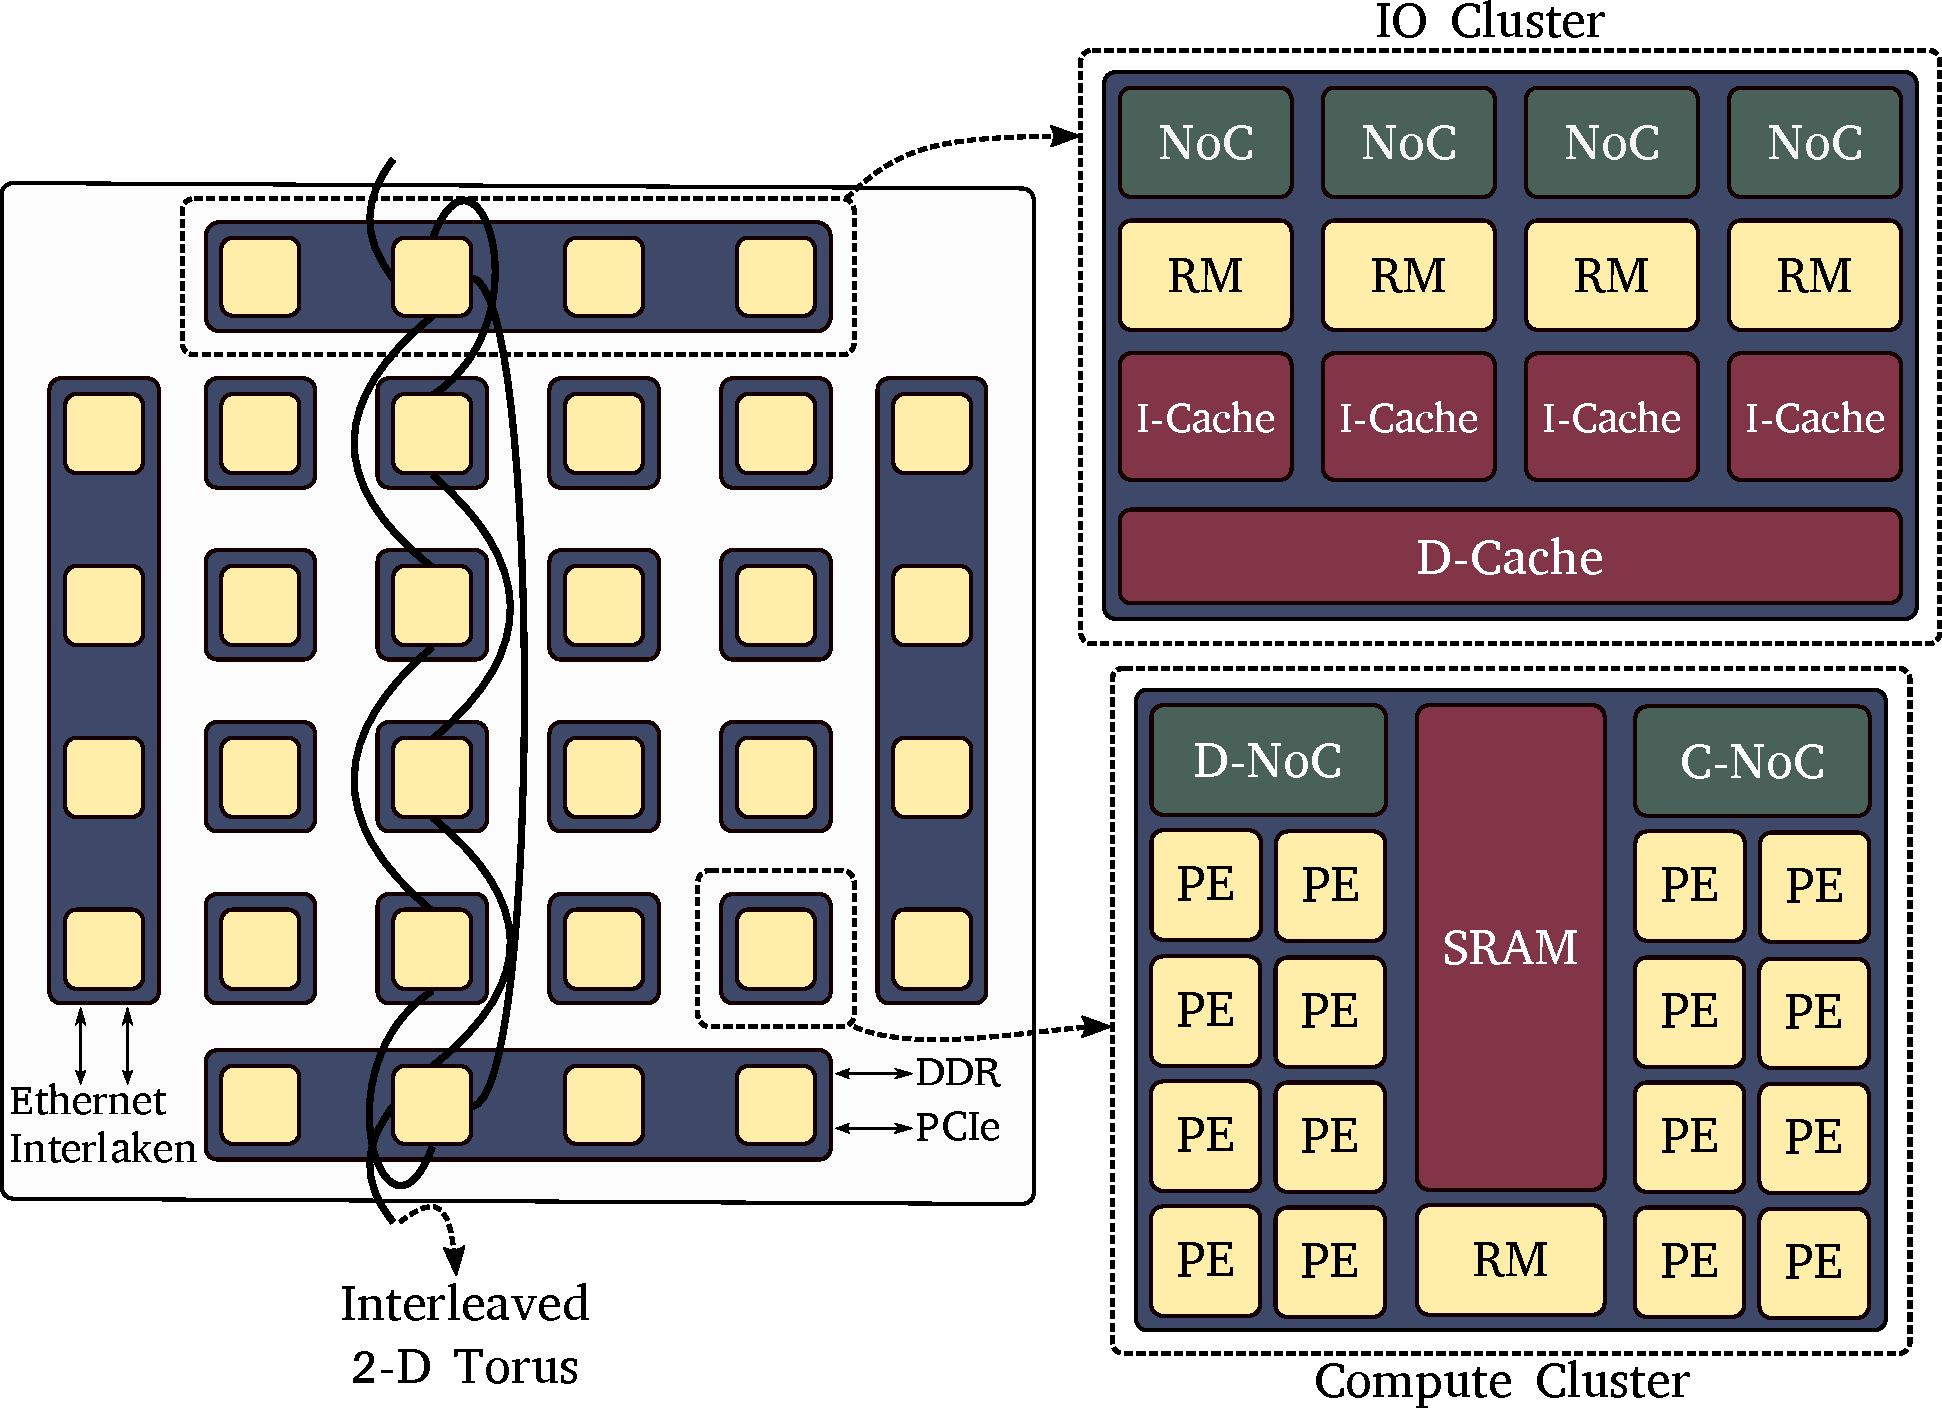
\includegraphics[width=7cm, keepaspectratio]{figs/mppa-overview.pdf}
\caption{Visão arquitetural simplificada do \mppa \cite{Penna2018}.}\par
\label{fig:mppaOverview}
\end{figure}

É importante salientar que ambos \ccs e \textit{clusters} de \io não podem acessar diretamente os dados armazenados na memoria interna de um outro \textit{cluster} que não ele mesmo. Logo, o processador possui um modelo de memória distribuído \cite{Castro-Souza-CCPE:2016, Podesta2018}. Esta característica, comum a alguns processadores \manycore, é fator desafiador para implementação de aplicações paralelas otimizadas no \mppa \cite{Castro-IA3-JPDC:2014}. Também vale informar que, neste trabalho, \textit{clusters} de \io virão a ser chamados de \textit{master} e \ccs virão a ser chamados de \textit{slaves}.

\subsection{\capb}
\label{subsec:capb}

O \capb é um \textit{benchmark} formado por 7 aplicações implementadas em C, diferindo na tecnologia de paralelismo utilizada dependendo da arquitetura alvo a ser testada. Atualmente, o \textit{benchmark} opera sobre arquiteturas x86, utilizando OpenMP e futuramente POSIX Threads. Também opera sobre o gem5 e o \mppa. O modulo voltado ao \mppa foi construído para testar todos os cenários de computação que este possa se deparar. Logo, as aplicações abrangem diversos problemas em diversos domínios, como grafos, ordenação e computação gráfica. Constituem o \capb os seguintes kernels: \textbf{(i)} Features from Accelerated Segment Test; \textbf{(ii)} Friendly Numbers; \textbf{(iii)} Gaussian Filter; \textbf{(iv)} Integer Sort; \textbf{(v)} K-Means; \textbf{(vi)} LU Factorization; e \textbf{(vii)} Traveling-Salesman Problem.

Originalmente, as aplicações voltadas ao o \mppa foram desenvolvidas explorando a \api \ipc, da Kalray. Esta \api, baseada no padrão POSIX \ipc, lida com comunicações entre \ccs, e entre \ccs e \textit{clusters} de \es. Ao usar a \ipc, é preciso lidar com paralelismo explicito, onde o programador implementa o comportamento do paralelismo e cada unidade de trabalho é independente em termos de dados e computação \cite{Castro-Souza-CCPE:2016}


\subsection{Comunicação assincrona}
\label{subsec:async}

Recentemente, a Kalray disponibilizou uma nova \api para comunicação assincrona e unilateral entre os \textit{clusters} do \mppa, a \async. Esta nova \api,

\begin{figure}[h]
\centering
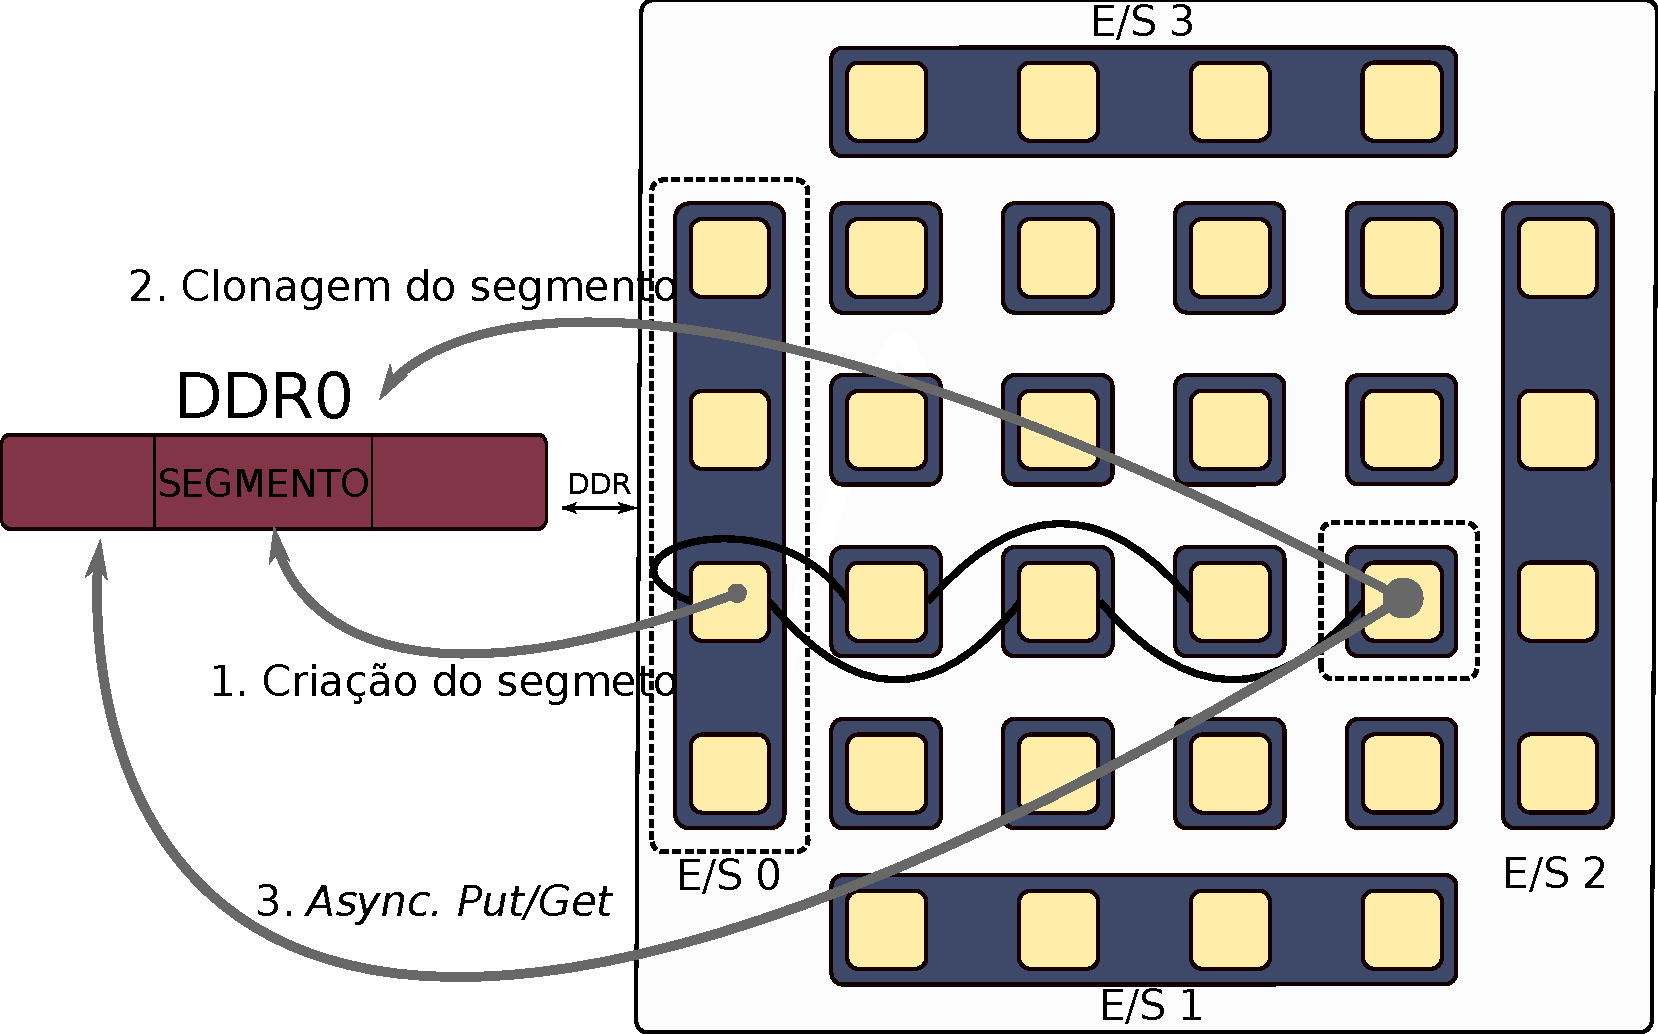
\includegraphics[width=7cm, keepaspectratio]{figs/putget.pdf}
\caption{Etapas da utilização da \api \async.}\par
\label{fig:asyncOverview}
\end{figure}


\subsection{Trabalhos Relacionados}

\section{Proposta e implementação de otimização no \capb}
\label{sec:capbMPPA}

Para a realização da otimização proposta, foi implementado, em todas as aplicações, uma nova logica de comunicação entre \textit{clusters} de \io e \ccs, e entre \ccs, onde o uso da \async substituiu por completo o uso da antiga \ipc. Como a nova \api simula um modelo de memoria compartilhado em suas operações, trabalhar com ela torna a tarefa de otimização consideravelmente mais fácil. Também são abrangidos, nesta nova lógica, diversas modificações sobre em qual tipo de \textit{cluster} é computado determinada operação de um \textit{kernel}, com objetivo de usufruir do poder de processamento dos \ccs, quando necessário, ou da memoria local dos \textit{clusters} de \io, onde inicializa-se o dado a ser trabalhado. Todas as alterações serão mostradas detalhadamente, para cada \textit{kernel}, nesta seção.

\subsection{Alterações no Friendly Numbers}
\label{subsec:async}

Primeiramente, foi alterado a implementação da função que calculava a soma de todos os divisores de um certo inteiro. Em sua versão antiga, esta função realizava a busca dos divisores no intervalo entre 2 e aquele inteiro. Já na otimizada, a busca é feita entre 2 e a metade deste inteiro, pois, acima da metade, sabemos que só existe ele como divisor de si mesmo. Quanto a utilização da \async, foi criado um segmento sobre o \textit{array} de itens a serem passados dos \textit{clusters} de \io para os \ccs, onde cada \cc possui um intervalo de \textit{offsets} no qual pode realizar operações sobre este segmento. Este intervalo é definido, em tempo de execução, no processo mestre no \textit{cluster} de \io, o qual repassa estas informações aos \textit{slaves} no momento que os inicializa.

\subsection{Alterações no LU Factorization}
\label{subsec:async}

Funções que setavam um novo pivô sobre a linha da matriz sendo iterada em algum \cc , realizando buscas por toda matriz e subsequentes trocas de linhas e colunas, foram removidas, pois, para calcular a fatoração LU não são permitidas tais operações, já que, ao realiza-las, é feito a decomposição PLU da matriz original, onde P é uma matriz de permutação. Além disso, a matriz L resultante não mais seria triangular inferior. Assim, sem as computações citadas acima, já é de se esperar ganho em desempenho enorme. Erros relacionados a passagem de tarefas dos \textit{clusters} de \io para os \ccs também foram arrumados, pois, na versão antiga, os blocos dentro da matriz eram passados aos \textit{slaves} desalinhados, gerando descontinuidade na informação e resultado final errôneo.

Para tirar proveito da \async neste \textit{kernel}, foi criado um segmento sobre a matriz original, representada por um \textit{array} unidimensional. Porém, diferentemente do FN, ao iniciar os \textit{slaves}, só é informado a eles o tamanho da matriz a ser decomposta. Auxiliar ao segmento da matriz, foi criado um segmento para conter os \textit{offsets} que serão utilizados pelos \ccs, no segmento da matriz, em uma certa iteração. É sobre este segmento que, em diversos momentos, cada \cc retira a informação sobre qual intervalo de \textit{offsets}, no segmento da matriz, ele deve pegar o dado. Não foi preciso informar aos \textit{slaves}, em sua inicialização, qual é seu \textit{offset} no segmento de \textit{offsets} visto que podemos utilizar seu próprio \textit{id} para isto.
\subsection{Alterações no K-Means}
\label{subsec:async}

Neste \textit{kernel}, diversas simplificações foram feitas. Primeiramente, para criar somente um segmento sobre a porção de dados a ser apurada e utilizar a \async de modo otimizado, foi necessário transformar o modelo de dados da aplicação. Antigamente, os pontos eram definidos como \textit{structs}, chamadas de vetores, contendo o tamanho (dimensão do vetor) e um ponteiro para os elementos (coordenadas do vetor). Porém, como todos os vetores possuem o mesmo tamanho, já que a dimensão é tratada globalmente, foi possível otimizar este modelo de dados, setando todos os pontos em um único \textit{array} unidimensional, o qual criou-se um segmento sobre. Vale salientar que a criação deste \textit{array} toma muito menos instruções do que a criação do \textit{array} de \textit{arrays} anterior. Desta maneira, em um cenário com $\mathnormal{P}$ pontos, todos com dimensão $\mathnormal{X}$, cada ponto ocupa $\mathnormal{X}$ posições do \textit{array} e o tamanho total deste é de $\mathnormal{X}$ $\times$ $\mathnormal{P}$ posições.

Para recalcular os \textit{centroids}, na antiga versão, toda a computação de calculo da distancia euclidiana média era feita nos \ccs. Isto requeria que os \ccs enviassem a informação sobre suas populações parciais para os \textit{clusters} de \io, os quais passariam de volta a soma destes dados a todos os \ccs. Já na nova, realizamos nos \ccs somente a primeira etapa deste calculo, a soma dos seus vetores parciais. Para calcular a média, necessitamos da população total, o que é mais facilmente disponível nos \textit{clusters} de \io após determinada iteração. Assim, geramos menos comunicação, mais especificamente, 3 operações \textit{GET} e 3 \textit{PUT}, ao contrario das 5 operações \textit{GET} e 5 \textit{PUT} da antiga versão.
\subsection{Alterações no Gaussian Filter}
\label{subsec:async}

\subsection{Alterações no Features from Accelerated Segment Test}
\label{subsec:async}

\subsection{Alterações no Integer Sort}
\label{subsec:async}

\section{Resultados}
\label{sec:resultados}

\section{Conclusão}
\label{sec:conclusao}



\section{Avaliação PIBIC: Benefícios e Formação Científica}

Este projeto de pesquisa contribuiu de inúmeras formas para minha formação acadêmica. Do começo ao fim foi algo engrandecedor e acredito que, ao longo da minha carreira profissional, irei utilizar diversos conhecimentos aqui adquiridos. Este foi o primeiro projeto no qual tive contato com uma documentação de \api, e, assim como nosso primeiro contato com qualquer tecnologia nova, foi bastante desafiador. Através de muita dedicação e ajuda do meu orientador e colegas de trabalho, consegui quebrar as barreiras do conhecimento e entender a fundo como funciona a nova \api da Kalray, a \async.  

Neste ciclo de pesquisa também produzi um artigo científico, o qual foi aprovado na decima nona Escola Regional de Alto Desempenho da Região Sul (ERAD/RS 2019), ocorrida na cidade de Três de Maio, no Rio Grande do Sul. Com esta aprovação, fui apresenta-lo nesta mesma cidade na data de realização do evento. Participar deste evento foi também uma experiencia enriquecedora, pois pude conhecer projetos de diferentes níveis de complexidade, englobando tanto projetos de iniciação cientifica quanto os do estado da arte.

Com este projeto de pesquisa pude também descobrir o que pretendo seguir na minha carreia profissional, assim como ter plena certeza de que de quero continuar com a pesquisa e contribuir de forma significativa para o avanço tecnológico de toda comunidade cientifica. Utilizarei também os resultados deste para realização do meu trabalho de conclusão de curso, onde pretendo expandir o que já foi pesquisado, realizando comparações com outros processadores do estado da arte.
 
\bibliography{bibliografia} 
\bibliographystyle{sbc}

\end{document}
